% Just The Docs Front Matter
% title: Inversions
% parent: Tutorials
% has_children: false
% has_toc: false

\subsection{Inversions} \label{sec:using-issm-tutorials-inversions}
\subsubsection{Goals} %{{{
\begin{itemize}
	\item Learn how to use the model to invert for ice rigidity (B) and basal friction from surface velocities
	\item Being able to choose the right cost functions, with the right weights
	\item Understand the limitations of inversions
\end{itemize}
%}}}

\subsubsection{Introduction}%{{{
Several model input parameters, such as the ice rigidity $B$ (\lstinlinebg|md.materials.rheology_B|) and basal friction $\alpha$ (\lstinlinebg|md.friction.coefficient|), are difficult to measure remotely and are critical controls on ice dynamics.

To get a good guess of what these parameters are, we use \emph{inversions}. Inversions consist in inferring unknown parameters using additional observations. Here, we use surface velocities to infer our unknown input parameters, by minimizing the misfit between the observed and modeled velocities.

For example, our cost function could be:
\begin{equation}
	{\mathcal J\left({\bf v}\right)}
	=\int_{S} \dfrac{1}{2}\left(
	\left(v_x-v_x^{\text{obs}}\right)^{2}
	+\left(v_y-v_y^{\text{obs}}\right)^{2}
	\right) dS
\end{equation}
And so we would optimize our unknown model input to minimize the cost function ${\mathcal J}$.

Inversions were first introduced to glaciology by \cite{MacAyeal1993a} for an SSA model, and extended since to 3D models for other model parameters.

To illustrate this method, we are going to perform a twin experiment. We give ourselves a rigidity field (B) and use the modeled velocities as synthetic observation in a second run, where we start from another initial rigidity field, and see if we can recover the rigidity field that was used to generate the observations.
%}}}
\subsubsection{Hands on 1 (ice rigidity, B)} %{{{
\paragraph{Step 1: Generating Observations}
First, go to \lstinlinebg|<ISSM_DIR>/examples/Inversion/| and start MATLAB. We will start by creating a new model and generate our synthetic observations. Open the \lstinlinebg|runme.m| and ensure that \lstinlinebg|step = 1| at the top of the file. Execute this first step:
\begin{lstlisting}
>> runme
\end{lstlisting}
You will see on the left our prescribed rigidity, $B$, and to the right the calculated velocities. We choose a pattern with 2 distinct values for $B$ for the upper left region, and stiffer ice for the lower right, with a sharp transition.
\begin{figure}[H]
	\begin{center}
		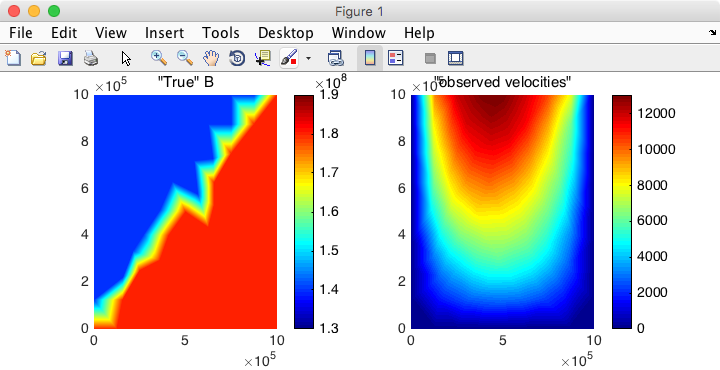
\includegraphics[width=\textwidth]{\assetsParentPath/assets/img/using-issm/tutorials/inversion/step1.png}
	\end{center}
\end{figure}
In the next step, we our going to change the rigidity to something uniform, use our previously calculated velocities (from step 1) as observations, and see if we can recover that initial pattern that was used to generate the observations.

\paragraph{Step 2: Initial guess and initial velocity}
We now change the rigidity, $B$, and make it uniform. The results of the previous step are taken as observations (but we will only use them in step 3). Open \lstinlinebg|runme.m| and set \lstinlinebg|step = 2|. Save the file and execute step 2 in MATLAB as above.
\begin{figure}[H]
	\begin{center}
		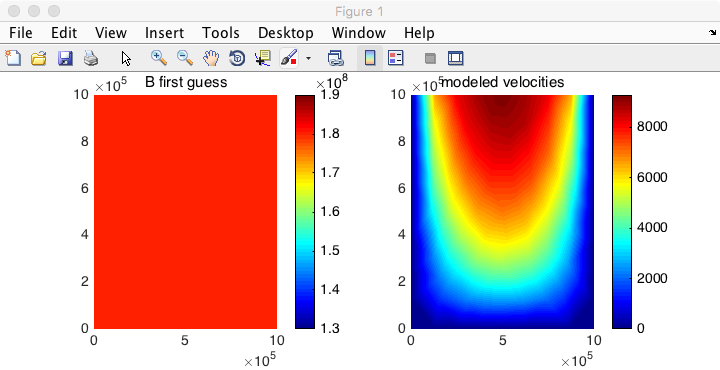
\includegraphics[width=\textwidth]{\assetsParentPath/assets/img/using-issm/tutorials/inversion/step2.png}
	\end{center}
\end{figure}
We now see that the left panel is constant, and the velocity is symmetrical. This is our initial guess for $B$ and our initial modeled velocity. In the next step, we are going to tune $B$, so that the modeled velocity is as close as possible to the velocity of step 1.

\paragraph{Step 3: Inverting for B}
We perform here the inversion of $B$. Open \lstinlinebg|runme.m| and set the step as \lstinlinebg|step = 3|.
\begin{figure}[H]
	\begin{center}
		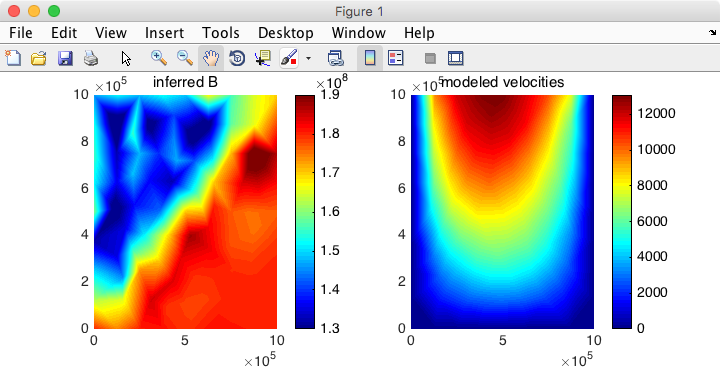
\includegraphics[width=\textwidth]{\assetsParentPath/assets/img/using-issm/tutorials/inversion/step3.png}
	\end{center}
\end{figure}
The general pattern is right (stiffer ice in the lower right), but it is noisy. Inverse problems are ill-posed: a solution might not exist, might not be unique, and might not depend continuously on input data. One of the consequences is that the inferred pattern for $B$ is not smooth, and these wiggles are \emph{not} physical. Adding regularization that penalizes wiggles in the control parameter stabilizes the inversion.

\paragraph{Step 4: Adding regularization}
Here, we would like to add a term of regularization to our cost function:
\begin{equation}
	{\mathcal J\left(B\right)}
	=
	\int_{S} w_1 \dfrac{1}{2}\left(
	\left(v_x-v_x^{\text{obs}}\right)^{2}
	+\left(v_y-v_y^{\text{obs}}\right)^{2}
	\right) dS
	+
	\int_{b} w_2 \dfrac{1}{2}
	\|\nabla B \|^{2}
	db
\end{equation}
The second term, known as Tikhonov regularization, penalizes strong gradients in $B$. Since the inversion tries to minimize our cost function $\mathcal J$, the optimization algorithm will try to also reduce the second term.

$w_1$ and $w_2$ are the weights associated to each component of the cost function. To have more regularization, one should increase $w_2$ (or decrease $w_1$), and vice versa.

Set \lstinlinebg|step = 4| in the \lstinlinebg|runme.m| file and execute it. Your results should now look like this:
\begin{figure}[H]
	\begin{center}
		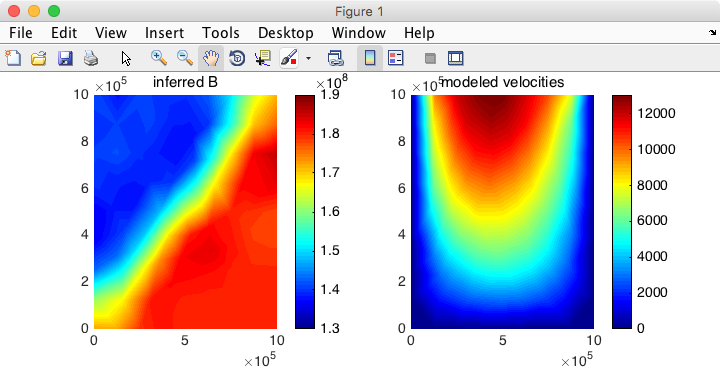
\includegraphics[width=\textwidth]{\assetsParentPath/assets/img/using-issm/tutorials/inversion/step4.png}
	\end{center}
\end{figure}
We successfully reconstructed the pattern of ice rigidity, but we could not capture the sharp transition between high and low rigidity because of the regularization that we had to introduce to stabilize the inversion.
%}}}
\subsubsection{Hands on 2 (friction)} %{{{
We would like to do the same twin experiment here, but invert for basal friction of a grounded glacier. Here, you are going to make additions and/or modifications to the \lstinlinebg|runme.m| script as described below.

\paragraph{Changes to step 1}
\begin{enumerate}
	\item The mask is now all grounded
	\item Increase bed (\lstinlinebg|md.geometry.base|) and surface elevation (\lstinlinebg|md.geometry.surface|) by 100 meters
	\item $B$ (\lstinlinebg|md.materials.rheology_B|) is now uniform = 1.8x10\textsuperscript{8}
	\item Friction coefficient: 50, and 10 for 400,000\verb|<|x\verb|<|600,000
	\item change the \lstinlinebg|plotmodel| command and plot \lstinlinebg|md.friction.coefficient| instead, between 0 and 100.
\end{enumerate}
After running step 1 again, you should get the following figure.
\begin{figure}[H]
	\begin{center}
		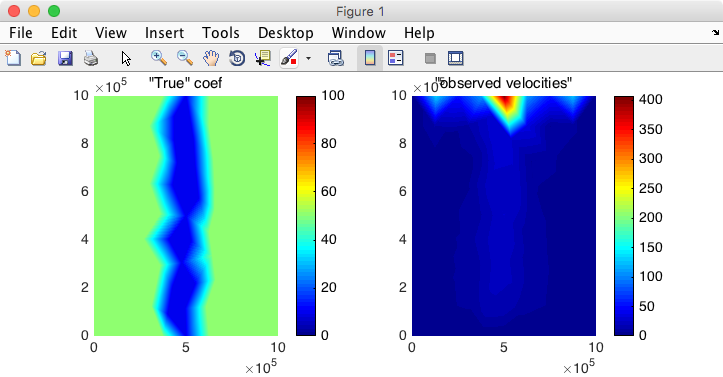
\includegraphics[width=\textwidth]{\assetsParentPath/assets/img/using-issm/tutorials/inversion/step1b.png}
	\end{center}
\end{figure}
If you don't, then double check your changes before looking at the solutions below. We are modeling here a glacier flowing over a region where there is a lot of sliding. We want to see if the inversion can reconstruct this region of low friction.

\paragraph{Solutions to step 1 (MATLAB)}
\begin{lstlisting}
%Generate observations
md = model;
md = triangle(md, 'DomainOutline.exp', 100000);

%CHANGES START
md = setmask(md, '', '');
%CHANGES END

md = parameterize(md, 'Square.par');

%CHANGES START
md.geometry.base = md.geometry.base + 100;
md.geometry.surface = md.geometry.surface + 100;
md.materials.rheology_B(:) = 1.8e8;
md.friction.coefficient(:) = 50;
pos = find(md.mesh.x > 400e3 & md.mesh.x < 600e3);
md.friction.coefficient(pos) = 10;
%CHANGES END

md = setflowequation(md, 'SSA', 'all');
md.cluster = generic('np', 2);
md = solve(md, 'Stressbalance');

%CHANGES START
plotmodel(md, 'axis#all', 'tight', 'data', md.friction.coefficient, 'caxis', [0 100], 'title', '"True" coef', ...
   'data', md.results.StressbalanceSolution.Vel, 'title', '"observed velocities"')
%CHANGES END

save model1 md
\end{lstlisting}

\paragraph{Solutions to step 1 (Python)}
\begin{lstlisting}
import numpy as np
from model import *
from setmask import setmask
from parameterize import parameterize
from setflowequation import setflowequation
from generic import generic
from solve import solve
from plotmodel import plotmodel
from export_netCDF import export_netCDF
from m1qn3inversion import m1qn3inversion
from verbose import verbose
from loadmodel import loadmodel
from cuffey import cuffey

steps = [5]
Clims = [1.3 * 1e8, 1.9 * 1e8]

if 1 in steps:
    #Generate observations
    md = model()
    md = triangle(md, 'DomainOutline.exp', 100000)
    #CHANGES START
    md = setmask(md, '', '')
    #CHANGES END
    md = parameterize(md, 'Square.py')
    #CHANGES START
    md.geometry.base = md.geometry.base + 100.
    md.geometry.surface = md.geometry.surface + 100.
    md.friction.coefficient[:] = 50
    pos = np.nonzero(np.logical_and(md.mesh.x > 400e3, md.mesh.x < 600e3))
    md.friction.coefficient[pos] = 10
    #CHANGES END

    md = setflowequation(md, 'SSA', 'all')
    md.cluster = generic('np', 2)
    md = solve(md, 'Stressbalance')
    #CHANGES START
    plotmodel(md, 'axis#all', 'tight', 'data', md.friction.coefficient, 'caxis', [0, 100], 'title', '"True" coef', 'data', md.results.StressbalanceSolution.Vel, 'title', '"observed velocities"')
    #CHANGES END

    export_netCDF(md, 'model1.nc')

if 2 in steps:
    #Modify rheology, now constant
    md = loadmodel('model1.nc')
    md.materials.rheology_B[:] = 1.8 * 1e8

    #results of previous run are taken as observations
    md.inversion = m1qn3inversion()
    md.inversion.vx_obs = md.results.StressbalanceSolution.Vx
    md.inversion.vy_obs = md.results.StressbalanceSolution.Vy
    md.inversion.vel_obs = md.results.StressbalanceSolution.Vel

    #CHANGES START
    md.friction.coefficient[:] = 50
    #CHANGES END

    md = solve(md, 'Stressbalance')
    #CHANGES START
    plotmodel(md, 'axis#all', 'tight', 'data', md.friction.coefficient, 'caxis', [0, 100], 'title', '"True" coef', 'data', md.results.StressbalanceSolution.Vel, 'title', '"observed velocities"')
    #CHANGES END
    export_netCDF(md, 'model2.nc')

if 3 in steps:
    #invert for ice rigidity
    md = loadmodel('model2.nc')

    #Set up inversion parameters
    maxsteps = 20
    md.inversion.iscontrol = 1
    #CHANGES START
    md.inversion.control_parameters = ['FrictionCoefficient']
    #CHANGES END
    md.inversion.maxsteps = maxsteps
    md.inversion.cost_functions = [101]
    md.inversion.cost_functions_coefficients = np.ones((md.mesh.numberofvertices, 1))
    #CHANGES START
    md.inversion.min_parameters = np.ones((md.mesh.numberofvertices, 1))
    md.inversion.max_parameters = 100. * np.ones((md.mesh.numberofvertices, 1))
    #CHANGES END

    #Go solve!
    md.verbose = verbose(0)
    md = solve(md, 'Stressbalance')
    #CHANGES START
    plotmodel(md, 'axis#all', 'tight', 'data', md.results.StressbalanceSolution.FrictionCoefficient, 'caxis', [0, 100], 'title', '"True" coef', 'data', md.results.StressbalanceSolution.Vel, 'title', '"observed velocities"')
    #CHANGES END

if 4 in steps:
    #invert for ice rigidity
    md = loadmodel('model2.nc')

    #Set up inversion parameters
    maxsteps = 20
    md.inversion.iscontrol = 1
    md.inversion.control_parameters = ['FrictionCoefficient']
    md.inversion.maxsteps = maxsteps
    #CHANGES START
    md.inversion.cost_functions = [101, 103]
    md.inversion.cost_functions_coefficients = np.ones((md.mesh.numberofvertices, 2))
    md.inversion.cost_functions_coefficients[:, 0] = 3000
    md.inversion.cost_functions_coefficients[:, 1] = 1
    #CHANGES END
    md.inversion.min_parameters = np.ones((md.mesh.numberofvertices, 1))
    md.inversion.max_parameters = 100. * np.ones((md.mesh.numberofvertices, 1))

    #Go solve!
    md.verbose = verbose(0)
    md = solve(md, 'Stressbalance')
    #CHANGES START
    plotmodel(md, 'axis#all', 'tight', 'data', md.results.StressbalanceSolution.FrictionCoefficient, 'caxis', [0, 100], 'title', '"True" coef', 'data', md.results.StressbalanceSolution.Vel, 'title', '"observed velocities"')
    #CHANGES END

if 5 in steps:
    #invert for ice rigidity
    md = loadmodel('model2.nc')

    #Set up inversion parameters
    maxsteps = 20
    md.inversion.iscontrol = 1
    md.inversion.control_parameters = ['FrictionCoefficient']
    md.inversion.maxsteps = maxsteps
    #CHANGES START
    md.inversion.cost_functions = [101, 103, 501]
    md.inversion.cost_functions_coefficients = np.ones((md.mesh.numberofvertices, 3))
    #CHANGES END
    md.inversion.cost_functions_coefficients[:, 0] = 3000
    md.inversion.cost_functions_coefficients[:, 1] = 1
    #CHANGES START
    md.inversion.cost_functions_coefficients[:, 2] = 0.01
    #CHANGES END
    md.inversion.min_parameters = np.ones((md.mesh.numberofvertices, 1))
    md.inversion.max_parameters = 100. * np.ones((md.mesh.numberofvertices, 1))

    #Go solve!
    md.verbose = verbose(0)
    md = solve(md, 'Stressbalance')
    plotmodel(md, 'axis#all', 'tight', 'data', md.results.StressbalanceSolution.FrictionCoefficient, 'caxis', [0, 100], 'title', 'inferred B', 'data', md.results.StressbalanceSolution.Vel, 'title', 'modeled velocities')
\end{lstlisting}

\paragraph{Changes to step 2}
For step 2, we now want to set our new first guess for the basal friction to a uniform value.
\begin{enumerate}
	\item set the friction (\lstinlinebg|md.friction.coefficient|) to a uniform value of 50
	\item change the \lstinlinebg|plotmodel| command and plot \lstinlinebg|md.friction.coefficient| instead, between 0 and 100.
\end{enumerate}
After running step 2, you should get the following figure:
\begin{figure}[H]
	\begin{center}
		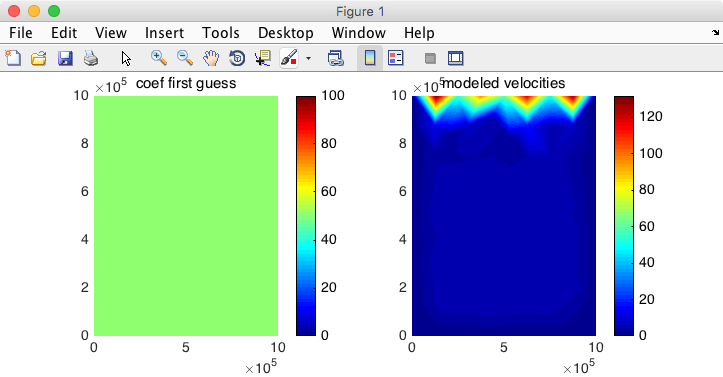
\includegraphics[width=\textwidth]{\assetsParentPath/assets/img/using-issm/tutorials/inversion/step2b.png}
	\end{center}
\end{figure}
if you don't, double check your changes. As you can see, the velocity does not show any fast flowing ice stream in the center of the domain, as expected since the friction is uniform.

\paragraph{Solutions to step 2}
\begin{lstlisting}
%Modify rheology, now constant
loadmodel('model1.mat');
md.materials.rheology_B(:) = 1.8 * 10^8;

%results of previous run are taken as observations
md.inversion = m1qn3inversion();
md.inversion.vx_obs		= md.results.StressbalanceSolution.Vx;
md.inversion.vy_obs		= md.results.StressbalanceSolution.Vy;
md.inversion.vel_obs	= md.results.StressbalanceSolution.Vel;

%CHANGES START
md.friction.coefficient(:) = 50;
%CHANGES END

md = solve(md, 'Stressbalance');
%CHANGES START
plotmodel(md, 'axis#all', 'tight', 'data', md.friction.coefficient, 'caxis', [0 100], 'title', 'coeff first guess', ...
	'data', md.results.StressbalanceSolution.Vel, 'title', 'modeled velocities')
%CHANGES END
save model2 md
\end{lstlisting}

\paragraph{Changes to step 3}
We now want to invert for basal friction and see if we can reconstruct the zone of sliding. We need to change what we are inverting for, and change the optimization parameters:
\begin{itemize}
	\item We now invert for \lstinlinebg|'FrictionCoefficient'|
	\item Do we keep the same cost function? yes for now...
	\item We want the parameter to be between 1 and 100
\end{itemize}
After running step 3, you should get the following figure:
\begin{figure}[H]
	\begin{center}
		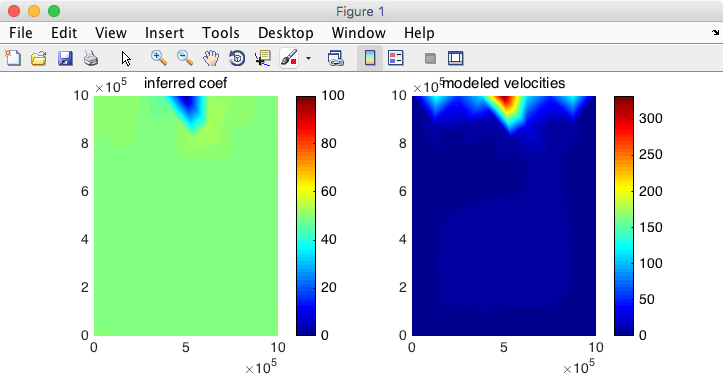
\includegraphics[width=\textwidth]{\assetsParentPath/assets/img/using-issm/tutorials/inversion/step3b.png}
	\end{center}
\end{figure}
if you don't, the solutions are as follows,

\paragraph{Solutions to step 3}
\begin{lstlisting}
%invert for ice rigidity
loadmodel('model2.mat');

%Set up inversion parameters
maxsteps = 20;
md.inversion.iscontrol = 1;
%CHANGES START
md.inversion.control_parameters = {'FrictionCoefficient'};
%CHANGES END
md.inversion.maxsteps = maxsteps;
md.inversion.cost_functions = 101;
md.inversion.cost_functions_coefficients = ones(md.mesh.numberofvertices, 1);
%CHANGES START
md.inversion.min_parameters = ones(md.mesh.numberofvertices, 1);
md.inversion.max_parameters = 100*ones(md.mesh.numberofvertices, 1);
%CHANGES END

%Go solve!
md.verbose = verbose(0);
md = solve(md, 'Stressbalance');
%CHANGES START
plotmodel(md, 'axis#all', 'tight', 'data', md.results.StressbalanceSolution.FrictionCoefficient, 'caxis' , [0 100], 'title', 'inferred coeff', ...
	'data', md.results.StressbalanceSolution.Vel, 'title', 'modeled velocities')
%CHANGES END
\end{lstlisting}

As you can see, we get more sliding close to the front, but the rest of the domain is unchanged. That's because when we look at the velocity (right), it does capture the fast spot close to the front, so in terms of cost function, the inversion did a great job in matching the observation. But if we look at the log of the velocity (note, we are adding one to avoid \lstinlinebg|log(0)|):
\begin{lstlisting}
plotmodel(md, 'data', md.inversion.vel_obs + 1, 'data', md.results.StressbalanceSolution.Vel + 1, 'log#all', 10, 'caxis#all', [1 400])
\end{lstlisting}
\begin{figure}[H]
	\begin{center}
		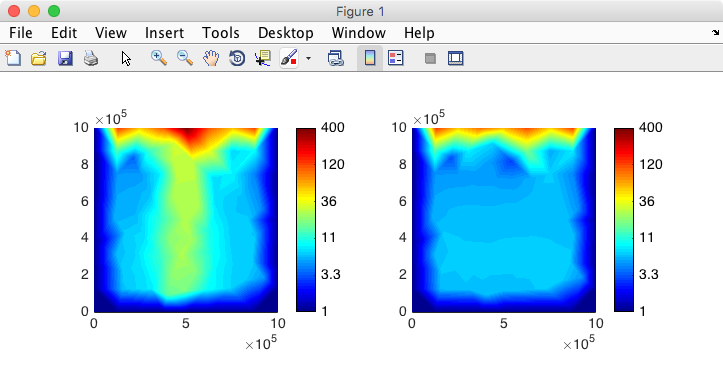
\includegraphics[width=\textwidth]{\assetsParentPath/assets/img/using-issm/tutorials/inversion/step3b_log.png}
	\end{center}
\end{figure}
we clearly see the zone of fast sliding in the observations but not in the results from the inversion. So we need to change the cost function to add this information, we not only want the square of the difference between modeled and observed velocities to be minimized, we also want their logs to be minimized.

\paragraph{Changing the cost function}
We want the cost function to include an additional term:
\begin{equation}
	{\mathcal J\left({\bf v}\right)}
	=\int_{S} w_1 \dfrac{1}{2}\left(
	\left(v_x-v_x^{\text{obs}}\right)^{2}
	+\left(v_y-v_y^{\text{obs}}\right)^{2}
	\right) dS
	+\int_{S} w_2 \left(\text{log}\left(
	\dfrac{\|{\bf v}\|+\varepsilon}{\|{\bf v}^{\text{obs}}\|+\varepsilon}
	\right) \right)^2 dS
\end{equation}
The 
%__@LATEX_ONLY_START@__
\hyperref[sec:using-issm-advanced-inversions]{`Advanced Features' $\rightarrow$ `Inversions' page}
%__@LATEX_ONLY_END@__
%__@MARKDOWN_ONLY_START@__
%<a href="../advanced/inversions">'Advanced Features' &#8594; 'Inversions' page</a>
%__@MARKDOWN_ONLY_END@__
lists all the cost function available. We want here the cost function to include the absolute and relative misfits. Typing in MATLAB \lstinlinebg|md.inversion| will give you the numbers associated to these cost function: \lstinlinebg|[101, 103]|. We also need to determine the weights associated to each cost function: $w_1$ and $w_2$. As a rule of thumb, it is generally preferable if the two components have the same order of magnitude at the end of the optimization. You can try with $w_1=w_2=1$ and run the inversion, look at their contribution at the end of the inversion and increase (or decrease) $w_1$. You need to change the following in step 3:
\begin{enumerate}
	\item We now want the cost functions 101 and 103
	\item the coefficients applied to each component of the cost functions has 2 columns (since there are 2 components)
	\item We want to increase $w_1$ to 3000
\end{enumerate}
You should get the following results:
\begin{figure}[H]
	\begin{center}
		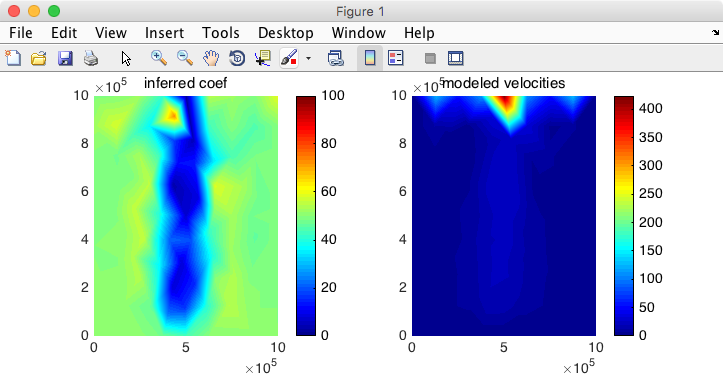
\includegraphics[width=\textwidth]{\assetsParentPath/assets/img/using-issm/tutorials/inversion/step3c.png}
	\end{center}
\end{figure}
The solutions are below if you don't have the same figure. We now successfully reconstructed the zone of sliding! But again, the pattern is a little bit noisy, and we are going to add regularization.

\paragraph{Solutions to step 3b}
\begin{lstlisting}
%invert for ice rigidity
loadmodel('model2.mat');

%Set up inversion parameters
maxsteps = 20;
md.inversion.iscontrol = 1;
md.inversion.control_parameters = {'FrictionCoefficient'};
md.inversion.maxsteps = maxsteps;
%CHANGES START
md.inversion.cost_functions = [101 103];
md.inversion.cost_functions_coefficients = ones(md.mesh.numberofvertices, 2);
md.inversion.cost_functions_coefficients(:, 1) = 3000;
md.inversion.cost_functions_coefficients(:, 2) = 1;
%CHANGES END
md.inversion.min_parameters = ones(md.mesh.numberofvertices, 1);
md.inversion.max_parameters = 100 * ones(md.mesh.numberofvertices, 1);

%Go solve!
md.verbose=verbose(0);
md = solve(md, 'Stressbalance');
%CHANGES START
plotmodel(md, 'axis#all', 'tight', 'data', md.results.StressbalanceSolution.FrictionCoefficient, 'caxis', [0 100], 'title', 'inferred coeff', ...
	'data', md.results.StressbalanceSolution.Vel, 'title', 'modeled velocities')
%CHANGES END
\end{lstlisting}

\paragraph{Adding regularization}
We want the cost function to include a regularization term:
\begin{equation}
	{\mathcal J}
	=\int_{S} w_1 \dfrac{1}{2}\left(
	\left(v_x-v_x^{\text{obs}}\right)^{2}
	+\left(v_y-v_y^{\text{obs}}\right)^{2}
	\right) dS
	+\int_{S} w_2 \left(\text{log}\left(
	\dfrac{\|{\bf v}\|+\varepsilon}{\|{\bf v}^{\text{obs}}\|+\varepsilon}
	\right) \right)^2 dS
	+\int_{B} w_3
	\dfrac{1}{2} \|\nabla \alpha \|^{2}
	dB
\end{equation}
You need to change the following in step 3:
\begin{enumerate}
	\item We now want the cost functions 101, 103 and 501
	\item the coefficients applied to each component of the cost functions has 3 columns (since there are 3 components)
	\item We want to set $w_3$ to 0.01
\end{enumerate}
You should get the following results:
\begin{figure}[H]
	\begin{center}
		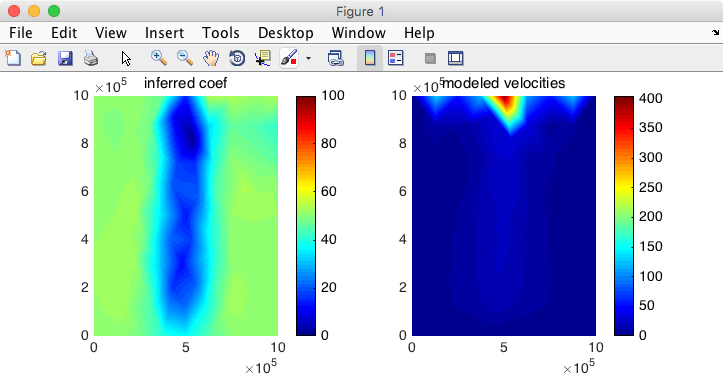
\includegraphics[width=\textwidth]{\assetsParentPath/assets/img/using-issm/tutorials/inversion/step4b.png}
	\end{center}
\end{figure}
The zone of sliding is captured and the inferred friction is smooth!

\paragraph{Solutions to step 3c}
\begin{lstlisting}
%invert for ice rigidity
loadmodel('model2.mat');

%Set up inversion parameters
maxsteps = 20;
md.inversion.iscontrol = 1;
md.inversion.control_parameters = {'FrictionCoefficient'};
md.inversion.maxsteps = maxsteps;
%CHANGES START
md.inversion.cost_functions = [101 103 501];
md.inversion.cost_functions_coefficients = ones(md.mesh.numberofvertices, 3);
%CHANGES END
md.inversion.cost_functions_coefficients(:, 1) = 3000;
md.inversion.cost_functions_coefficients(:, 2) = 1;
%CHANGES START
md.inversion.cost_functions_coefficients(:, 3) = 0.01;
%CHANGES END
md.inversion.min_parameters = ones(md.mesh.numberofvertices, 1);
md.inversion.max_parameters = 100 * ones(md.mesh.numberofvertices, 1);

%Go solve!
md.verbose = verbose(0);
md = solve(md, 'Stressbalance');
plotmodel(md, 'axis#all', 'tight', 'data', md.results.StressbalanceSolution.FrictionCoefficient, 'caxis', [0 100], 'title', 'inferred coeff', ...
	'data', md.results.StressbalanceSolution.Vel, 'title', 'modeled velocities')
\end{lstlisting}
%}}}

\clearpage % Make sure all figures are placed before next section
